L'applicativo si basa su tecnologie e servizi ampiamente adottati e consolidati in ambiente aziendale:

\section{RabbitMQ}
% Link utili
% https://www.ibm.com/it-it/topics/message-brokers
%
Rabbit \`e un message broker, cio\`e, un software che consente la comunicazione asincrona tra programmi.
Funziona attraverso \textit{queues} (code) su cui i \textit{producers} (mittenti) inviano messaggi definiti a priori,
e i \textit{consumers} (destinatari) consumano questi messaggi eseguendo operazioni in base al loro contenuto.
Rabbit in particolare utilizza gli \textit{exchange}, un punto intermedio tra i producer e le queues.
L'exchange riceve i messaggi dei producers e li instrada confrontando la \textit{routing key} del messaggio con determinate regole dette \textit{bindings}.\\\\
%
Rabbit ha diversi punti di forza, alcuni intrinsechi del tipo di software di cui fa parte, altri per via delle sue caratteristiche specifiche:\
\begin{itemize}
  \item \textbf{Scalabilit\`a} -  Il carico di lavoro viene distribuito automaticamente tra i consumer, e finch\'e i messaggi
    non vengono processati questi rimangono in coda.
  \item \textbf{Flessibilit\`a nel routing dei messaggi} - Rabbit offre molteplici modi di configurare gli exchange a seconda delle esigenze:
    \begin{enumerate}
      \item \textit{Direct Exchange} - Invio dei messaggi a code specifiche in base a una routing key
        \begin{figure}[H]
          \centering
          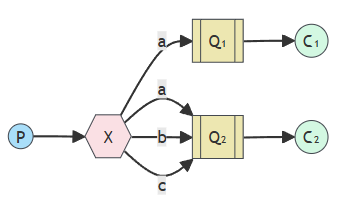
\includegraphics[width=5cm]{images/rabbitmq-direct-exchange.png}
          \caption{Esempio di Direct Exchange\cite{rabbitmq}}
        \end{figure}
      \item \textit{Fanout Exchange} - Invio su tutte le code appartenenti all'exchange, utile per il broadcasting
      \item \textit{Topic Exchange} - Permette di instradare i messaggi facendo il match delle routing key con binding basati su pattern pi\`u o meno complessi
        \begin{figure}[H]
          \centering
          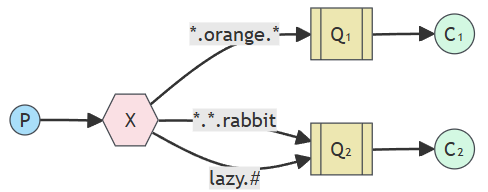
\includegraphics[width=7cm]{images/rabbitmq-topic-exchange.png}
          \caption{Esempio di Topic Exchange\cite{rabbitmq}}
        \end{figure}
      \item \textit{Header Exchange} - Utile per instradare i messaggi in base a molteplici argomenti, per esempio \`e possibile creare una coda
        che riceve messaggi con header ``format=pdf''
    \end{enumerate}
  \item \textbf{Affidabilit\`a} -  Rabbit \`e in grado di offrire un elevato grado di affidabilit\`a grazie a  molteplici meccanismi:
    \begin{enumerate}
      \item
        \textit{Acknowledgements} -  Una conferma da parte del consumer che tutto sia andato a buon fine.
        Se il consumer non invia l'ack, Rabbit terr\`a il messaggio all'interno della coda o lo invier\`a ad un altro consumer.
      \item \textit{TTL (Time-to-Live) per messaggi e code} - \`E possibile impostare un limite di tempo che un messaggio pu\`o rimanere
        in una queue, dopo il quale vengono automaticamente scartati o vengono spostati su un DLX, riducendo il rischio che si
        possano accumulare messaggi causando problemi di risorse esaurite o code sovraccariche.
      \item \textit{DLX (Dead-letter Exchange)} - Sono normali exchange su cui vengono inviati i messaggi \textit{``dead-lettered''}: messaggi che hanno
        ricevuto un nack (\textit{negative acknowledgement}), messaggi che hanno superato il TTL definito per messaggio, messaggi
        scartati perch\`e la queue ha superato uno dei limiti imposti, o messaggi che hanno superato il numero massimo di re-try consentito dalla coda.
      \item \textit{Persistenza dei messaggi} -  \`e possibile persistere i messaggi presenti nelle queue sul disco,
        che significa che questi non vengono persi al riavvio o al crash del server. La persistenza pu\`o essere attivata sia sulle code che sui singoli messaggi.
        Il contro della persistenza \`e che aumenta la latenza, ma offre ovviamente una maggiore affidabilit\`a.
    \end{enumerate}
\end{itemize}

\section{PostgreSQL}
Placeholder
\section{Java}
Placeholder
\subsection {SpringBoot}
Placeholder
\section{Angular}
Placeholder
\section{Stripe}
Placeholder
\section{Docker}
Placeholder
\subsection{Kubernetes}
Placeholder
